
\section{Übung 1}

\subsection{Aufgabe 1}

\begin{center}
\begin{tabular}{lcccr}
\textbf{Chiffre} & \textbf{Alphabet} & \textbf{Geheimtext} & \textbf{Schlüsselraum} & \textbf{Länge}                                  \\   \hline
Caesar  & $\{A, \cdots, Z \}$ & $\{A, \cdots, Z \}$ & $\{3\}, \{1, \cdots, 25 \}$ & 4,64     \\   \hline
OTP  	& $\{0,1 \}$  		  & $\{0,1 \}$      	& $\{0,1\}^*$ 				  & $\infty$ \\   \hline
DES  	& $\{0,1 \}$   		  & $\{0,1 \}$ 			& $\{0,1\}^{56}$ 		      & 56       \\   \hline
\end{tabular}
\end{center}
\subsection{Aufgabe 2}
\subsubsection{Beweis: Äquivalenzrelation: $\equiv_n$  }
\paragraph{Reflexivität}
\hspace{1cm} $ \forall x: x \equiv_n x $

\begin{equation}
	x \mod n \equiv r = x \mod n \imp x \equiv_{n} x 
\end{equation}
\qed

\paragraph{Symmetrie}
\hspace{1cm} $ \forall x,y: x \equiv_n y \imp y \equiv_n x $

\begin{align*}
	x \equiv_n y \mod n        
	& \imp 	x \mod n = r = y \mod n      \\ 
	& \imp	y \mod n = x \mod n        \imp  y \equiv_n x
\end{align*}
\qed


\paragraph{Transitiviät}
\hspace{1cm} $ \forall x,y,z: x \equiv_n y , y \equiv_n z => x \equiv_n z $

\begin{align*}
	n. V. & x \mod n = r_x,  										 \\
          & y \mod n = r_y  			   					     		 \\
          & z \mod n = r_z 										
           \wedge r_x = r_y , r_y=r_z \imp                           \\
		  & r_x = r_z \imp x \equiv_n z \mod n
\end{align*}
\qed

\subsubsection{}
\paragraph{} 
\hspace{1cm} \textbf{z.~Z.} $ [i]_n + [j]_n = [i+j]_n$

\begin{align*}
\text{Sei } a,b \in \INT &\imp a = q_an+r_a , b = q_bn+r_b    			 \\ \\
				 &\imp  a \in [r_a]_n , b \in  [r_b]_n  			     \\
				 &\imp [r_a]_n + [r_b]_n = \{ \forall i: in(r_a+r_b) \}	 \\
				 &\imp a + b =  q_an+r_a + q_bn+r_b                      \\
				 & \equiv_n   n(q_a+q_b)+r_a+r_b                   \\
				 & \equiv_n r_a+r_b  \imp [r_a+r_b]_n
\end{align*}

\paragraph{} 
\hspace{1cm} \textbf{z.~Z.} $ [i]_n \cdot [j]_n = [i \cdot j]_n$
\begin{align*}
\text{Sei } a,b \in \INT & \imp a = q_an+r_a , b = q_bn+r_b    			 \\ \\
				 &\imp  a \in [r_a]_n , b \in  [r_b]_n  			     \\
				 &\imp [r_a]_n * [r_b]_n = \{ \forall i: in(r_a*r_b) \}	 \\
				 &\imp a * b \equiv_n  (q_an+r_a) * (q_bn+r_b)                  \\
				 & \equiv_n  q_aq_bn+q_anr_b+q_bnr_a+r_a*r_b                   \\
				 & \equiv_n  n(q_aq_b+q_ar_b+q_br_a)+r_a*r_b                   \\				 
				 & \equiv_n r_a*r_b  =  [r_a+r_b]_n
\end{align*}

\subsection{}
\subsubsection{}
\begin{align*}
 ( 23.145 \cdot = 12.479 + 14.543 ) \cdot \mod 9 & \equiv_9 \\
 ( 6 \cdot 5 + 8 ) \cdot 5 & \equiv_9  3				    \\
 8 \cdot 5 &\equiv_9 \\
 2\cdot 5 \equiv_9 10 &= 1 \mod 9 
\end{align*}

\subsubsection{}
\begin{align*}
 123 \cdot  (123.983 \cdot 789.345 + 676.345) mod 11 & \equiv_{11} \\
 2    \cdot  (2 \cdot 7 + 10) & \equiv_{11}   \\
 2 \cdot (14 + 10 ) & \equiv_{11}  4 \mod 11
\end{align*}


\subsection{}

\begin{center}
	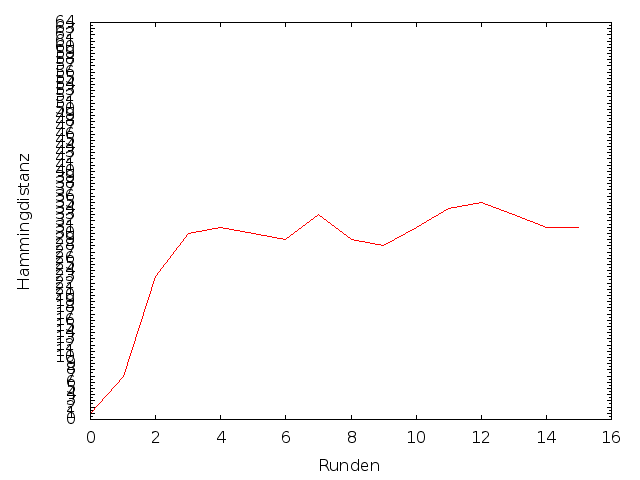
\includegraphics[scale=0.5]{images/ueb1_4.png}
\end{center}

\begin{table}[T]
\centering
\begin{tabular}{rr|rr}
Round $k$ & $HD(M_k,M_k)$ &  $HD(M_{1_k},M_{1_k})$ & $HD(M_{1_k},M_{1_k})$ \\ \hline
 0 &1 & 39 & 35 \\
 1 &7 &35 &31      \\
 2 &23 &32 &33     \\ 
 3 &30 &36 &35     \\
 4 &31 &37 &34     \\
 5 &30 &31 &34     \\
 6 &29 &26 &30     \\
 7 &33 &26 &26     \\
 8 &29 &29 &26     \\
 9 &28 &29 &34     \\
10 &31 &25 &36     \\
11 &34 &28 &35     \\
12 &35 &30 &38     \\
13 &33 &29 &37     \\
14 &31 &32 &38     \\
15 &31
\\ \hline								
\end{tabular}
\end{table}